\section{What is a pointer?}
\begin{itemize}
    \item Some languages don't let you use pointers.
    \item In C there is no getting away from pointers.
    \item C is a low level language and this is why it let's you use pointers.
    \item So what is a pointer? A pointer is a variable that points to an address in memory.
    \item What is an address? Think of the computer memory as a large series of locations where data is stored, all of these locations are labled. A pointer is able to reference an address.
\end{itemize}

%%%%%%%%%%%%%%%%%%%%%%%%%%%%%%%%%%%%%%%%%%%%%%%%%%%%%%
\section{Pointer variables}
\begin{itemize}
    \item They are declared using the asterisk between the data type and the variable name.
\end{itemize}
\begin{figure}[H]
    \centering
    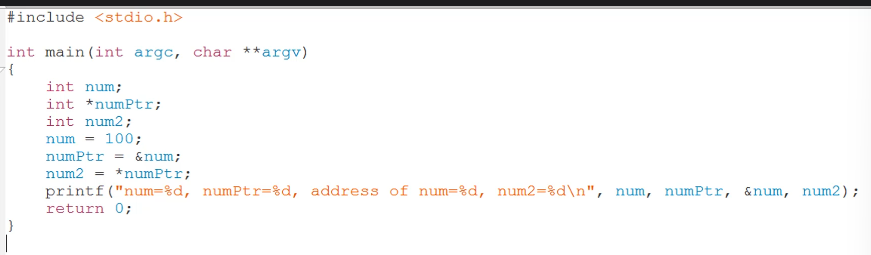
\includegraphics[width=\width\textwidth]{./figs/20220603204555.png}
    \caption{C program}
\end{figure}

%%%%%%%%%%%%%%%%%%%%%%%%%%%%%%%%%%%%%%%%%%%%%%%%%%%%%%
\section{Indirection}
\begin{itemize}
    \item If you have a pointer variable that hold the address in memory at which some other piece of data is stored, the address by itself is not really useful, but we can get the value in memory which is stored at the pointed location by using indirection or dereferncing.
    \item Given a pointer variable you can access the data being pointed to by adding an asterisk to the variable.
        \begin{figure}[H]
            \centering
            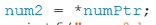
\includegraphics[width=\width\textwidth]{./figs/20220603204810.png}
            \caption{Indirection operation}
        \end{figure}
\end{itemize}

